\section{Current Exclusion Limits on Vector-Like Quarks}\label{sec:exp}

The ATLAS and CMS collaborations at CERN have conducted various searches for heavy vector-like quarks (T). These searches utilized $\mathrm{pp}$ collisions at center-of-mass energies of $\sqrt{s} = 8$ and $13$ \textrm{TeV}. The studies primarily focused on T production through gluon-mediated QCD processes, either in pair production from quark-antiquark annihilation (Fig.~\ref{fig:qcd_T_prod}) or in single-T production from electroweak processes involving associated quarks (Fig.~\ref{fig:qed_T_prod}). 

\begin{center}
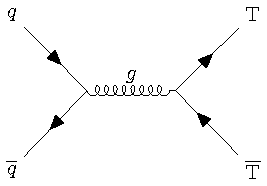
\includegraphics[width=0.6\linewidth]{Images/T_prod_qcd.pdf}
\captionof{figure}{Representative Feynman diagram for T pair production via gluon-mediated QCD processes.\label{fig:qcd_T_prod}}  
\end{center}

\begin{center}
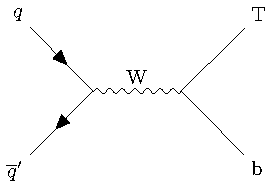
\includegraphics[width=0.6\linewidth]{Images/T_prod_qed.pdf}
\captionof{figure}{Representative Feynman diagram for single T production via electroweak processes.\label{fig:qed_T_prod}}  
\end{center}



In those studies, \textrm{T} decays into $\mathrm{bW}$, $\mathrm{tZ}$, or $\mathrm{tH}$ have been considered. In the context of \textrm{T} pair production, $\mathrm{T}\bar{\mathrm{T}}$, via QCD processes, the cross sections are well-known and solely depend on the mass of the vector-like quark.  Assuming a narrow $\mathrm{T}$ decay width ($\Gamma / m(\mathrm{T}) < 0.05$ or 0.1) and a 100\% branching fraction to $\textrm{bW}$, $\textrm{tZ}$, or $\textrm{tH}$, these searches have set stringent bounds on $m(\mathrm{T})$, excluding masses below almost 1.5 \textrm{TeV} at 95\% confidence level~\parencite{CMS:2024bni,CMS:2024qdd,ATLAS:2022ozf,ATLAS:2023bfh,ATLAS:2022hnn,ATLAS:2022tla,ATLAS:2023pja,ATLAS:2024fdw}. The most recent analysis from the CMS collaboration probes T-quark production via $\mathrm{pp} \to \mathrm{T}\textrm{qb}$, in final states with $\mathrm{T} \to \textrm{tZ}$ or $\mathrm{T} \to \textrm{tH}$, considering scenarios with preferential couplings to third-generation fermions. The analysis sets 95\% confidence level upper limits of 68-1260 \textrm{fb} on the production cross section, for T masses ranging from 600-1200 \textrm{GeV}~\parencite{CMS:2024qdd}. The latest studies from ATLAS probe vector-like quarks using the single-T production mode with the $\mathrm{T} \to \textrm{tH}$ decay channel leading to a fully hadronic final state~\parencite{ATLAS:2022ozf}, the single-T production mode with the $\mathrm{T} \to \textrm{tZ}$ decay channel leading to a multileptonic final state~\parencite{ATLAS:2023bfh}, the TT pair production mode with various T decay channels leading to multileptonic final states~\parencite{ATLAS:2022hnn}, and the TT pair production mode with various T decay channels leading to a single lepton plus missing momentum final state~\parencite{ATLAS:2022tla,ATLAS:2023pja}. 
The multilepton search offers the greatest sensitivity in most of the phase space, but the missing transverse energy based search has better sensitivity for low branching fraction $\mathfrak{B}(\mathrm{T}\to \textrm{Wb})$ and high $\mathfrak{B}(\mathrm{T}\to \textrm{Ht})$. These searches have similar sensitivities for the singlet and doublet models, resulting in exclusion bounds for masses below about 1.25 \textrm{TeV} and 1.41 \textrm{TeV}, respectively. 


A key consideration in the model interpretations summarized above is that the $\mathrm{T}$ branching fractions depend on the chosen model. The excluded mass range is less restrictive for specific branching fraction scenarios, such as $\{\mathfrak{B}(\mathrm{T} \to \textrm{tZ})$, $\mathfrak{B}(\mathrm{T} \to bW)$, $\mathfrak{B}(\mathrm{T} \to \textrm{tH})\}= \{0.2, 0.6, 0.2\}$, excluding masses below about 0.95 \textrm{TeV}. Moreover, if the $\mathrm{T} \to \phi't $ decay is allowed, or if the branching fractions $\mathfrak{B}(\mathrm{T} \to \textrm{tH/bW})$ are lower, the limits previously quoted must be re-evaluated. The authors of Ref.~\parencite{Cacciapaglia:2019zmj} emphasize that bounds on $m(\mathrm{T})$ can be around 500 \textrm{GeV} when $\mathrm{T} \to \mathrm{t}\phi'$ decays are permitted. Therefore, to facilitate a comprehensive study, benchmark scenarios in this paper are considered down to $m(\chi_\mathrm{u}) = 500$ \textrm{GeV}.
